\chapter{相关理论基础与关键技术}

实时流媒体拥塞控制系统的设计与优化，建立在底层网络通信协议与时序决策理论的交叉基础之上。本章旨在梳理本文研究依托的关键技术原理，剖析 WebRTC 底层传输机制及经典启发式拥塞控制算法的数学模型与固有局限，并在此基础上引入强化学习理论，系统推导隐式 Q 学习（Implicit Q-Learning, IQL）算法在应对离线学习分布偏移问题中的理论机制。

\section{WebRTC 实时通信机制与底层反馈框架}
\label{sec:webrtc-framework}
WebRTC 作为一个由 W3C 与 IETF 共同推动的开源实时通信标准，旨在为异构终端提供低延迟的点对点（P2P）媒体传输能力。其底层协议栈的复杂性体现在从信令握手、网络穿透到实时媒体流自适应传输的完整链路闭环中。
\subsection{协议栈架构与会话确立}
WebRTC 通信体系的建立依赖于高度标准化的协议集合。在信令阶段，终端通过应用层信令网关交换会话描述协议（Session Description Protocol, SDP），完成音视频编解码器规格及网络传输层属性的协商。由于实际通信节点普遍置于 NAT（网络地址转换）网关之后，系统需借助 ICE（Interactive Connectivity Establishment）框架，结合 STUN 与 TURN 服务器进行候选地址收集与连通性检查，从而确立最优的点对点 UDP 传输通道。媒体载荷与控制信令分别通过 SRTP（Secure Real-time Transport Protocol）和 RTCP（RTP Control Protocol）进行封装与传输。
\subsection{Transport-CC 反馈机制与状态观测}
在流媒体自适应传输层面，拥塞控制算法的有效性高度依赖于底层网络状态的精准观测。现代 WebRTC 架构普遍采用基于传输层范围的拥塞控制（Transport-wide Congestion Control, Transport-CC）扩展规范。与早期的接收端估算机制（如 REMB）不同，Transport-CC 将带宽预测的核心逻辑集中于发送端。
\par 具体而言，发送端在每个 RTP 数据包的扩展头部注入递增的传输层序列号。接收端不再进行复杂的带宽计算，仅负责记录每个序列号对应报文的物理到达时间（Arrival Time），并以极高的频率（通常为 20 毫秒至 100 毫秒量级）将这些时间戳信息打包进 RTCP 反馈报文（RTCP Feedback）中回传。发送端解包后，结合本地维护的报文发送时间记录，即可精确计算出当前链路的接收吞吐量、单向延迟梯度（Delay Gradient）以及实时丢包率。本文构建的数据采集与控制平台，正是通过挂载于此反馈回路之上的 API（如 getStats），实现对底层网络动力学特征的高频感知。

\section{RTC 拥塞控制建模与启发式算法演进}
拥塞控制的本质是分布式网络环境下的资源竞争与动态分配问题。在实时音视频交互（RTC）业务中，该问题表现出极强的多目标优化特性。
\subsection{拥塞控制的多目标优化模型}
有别于传统 TCP 协议以最大化吞吐量为单一诉求，RTC 拥塞控制要求在带宽利用率与传输时延之间寻找严格的平衡点。其综合体验质量（Quality of Experience, QoE）的效用函数通常可形式化表征为如下非线性组合：
$$QoE = f(R) - \alpha \cdot D - \beta \cdot L - \gamma \cdot \Delta R$$
式中，$R$ 代表目标发送码率，$f(R)$ 为码率带来的正向画质收益，常呈现对数型的边际递减特征；$D$ 表征包含排队时延在内的端到端延迟；$L$ 为网络丢包率；$\Delta R$ 代表相邻决策周期内码率波动的绝对值或方差；$\alpha$、$\beta$ 与 $\gamma$ 为对应的惩罚权重参数。高额的 $D$ 与 $L$ 会引发媒体播放的卡顿与重缓冲，而剧烈的 $\Delta R$ 则导致画面清晰度频繁闪烁。
\subsection{GCC 算法的耦合控制机制}
作为 WebRTC 默认的拥塞控制规范，Google 拥塞控制（Google Congestion Control, GCC）算法采用基于延迟（Delay-based）与基于丢包（Loss-based）的双回路耦合控制机制。
基于延迟的控制器旨在通过排队时延的变化趋势预判链路拥塞。其核心逻辑在于提取连续数据包组的发送时间差与到达时间差。当到达时间差持续大于发送时间差时，表征数据包在中间路由节点的缓冲区内发生堆积。GCC 利用卡尔曼滤波器（或趋势线滤波器）对延迟梯度进行平滑估计，并引入动态自适应阈值过滤瞬时噪声。依据过滤后的状态信号（Overuse、Underuse、Normal），控制器通过有限状态机输出乘性减或加性增的码率调节指令。
同时，基于丢包的控制器作为退后保护机制，直接响应 RTCP 反馈的丢包率 $p$：当 $p < 2\%$ 时判定网络闲置，允许码率上探；当 $p > 10\%$ 时强制触发乘性回退机制，即 $R_{new} = R_{old} \cdot (1 - 0.5p)$，以快速缓解严重拥塞。
\subsection{启发式规则在无线信道下的瓶颈}
尽管 GCC 算法的工程实现相对成熟，但在时变性强、拓扑复杂的无线接入网（如 Wi-Fi 竞争环境或蜂窝网络）中，其启发式规则设计暴露出了结构性缺陷。
一方面，无线信道衰落与介质访问控制（MAC）层的竞争极易引发非拥塞性的随机丢包（Random Loss）。GCC 的控制逻辑难以从观测中剥离此类噪声，常因误判拥塞而触发断崖式降速，致使带宽利用率严重恶化。另一方面，算法内置的趋势线斜率阈值及增减益系数多源于特定网络模型的经验调试。在面临长肥网络（大带宽大延迟）与浅缓存链路的场景切换时，静态参数无法动态适配信道容量的变化，使得算法在带宽骤变初期表现出显著的响应滞后与调节过冲，最终导致端到端延迟的恶化。

\section{强化学习理论与离线学习范式}
针对人工规则难以适配高维非平稳网络环境的问题，数据驱动的强化学习（Reinforcement Learning, RL）提供了一种旨在最大化长期累积奖励的自动决策框架。
\subsection{马尔可夫决策过程与在线 RL}
强化学习的理论内核为马尔可夫决策过程（Markov Decision Process, MDP），可由元组 $\langle \mathcal{S}, \mathcal{A}, P, r, \rho_0, \gamma \rangle$ 严格定义。在拥塞控制语境下，$\mathcal{S}$ 代表包含历史吞吐、延迟与丢包率的网络状态特征空间；$\mathcal{A}$ 为连续的目标码率动作空间；$P(s'|s,a)$ 表征网络信道的未知动态转移概率；$r(s,a)$ 即为前文定义的 QoE 奖励函数；$\gamma \in [0, 1)$ 为平衡远近收益的折扣因子。
\par 智能体的优化目标是寻得最优策略 $\pi^*(a|s)$，以最大化状态价值函数：
$$V^\pi(s) = \mathbb{E}_{\pi} \left[ \sum_{t=0}^{\infty} \gamma^t r(s_t, a_t) \Big| s_0 = s \right]$$
\par 传统在线强化学习（Online RL）要求智能体通过与环境的持续交互进行试错采样。然而，在真实的 RTC 生产系统中引入试错机制代价极高，探索初期的随机动作会直接摧毁用户的通信体验。若退而求其次在网络仿真器（如 ns-3）中进行在线训练，又不可避免地遭遇 Sim-to-Real（仿真至现实）的鸿沟。仿真器基于统计学假设的信道模型无法精确还原真实物理介质的微观抖动，导致仿真环境中收敛的策略在现网部署时往往面临鲁棒性崩塌。
\subsection{离线强化学习与分布偏移难题}
离线强化学习（Offline RL）为解决上述困境提供了一种纯数据驱动的范式。其核心约束在于：禁止智能体与环境进行任何形式的在线交互，策略学习仅能依赖一个由未知行为策略（Behavior Policy, $\pi_\beta$）预先采集的静态数据集 $\mathcal{D} = \{(s, a, r, s')\}$。这使得复用海量历史 GCC 运行日志进行零风险模型训练成为可能。
\par 然而，离线学习范式引入了严峻的分布偏移（Distributional Shift）挑战。基于贝尔曼最优方程的时序差分更新依赖于自举（Bootstrapping）操作：
$$Q(s,a) \leftarrow r + \gamma \max_{a'} Q(s', a')$$
\par 在拟合 $Q(s,a)$ 时，一旦策略试图评估数据集中未曾覆盖的分布外（Out-of-Distribution, OOD）动作 $a'$，神经网络不可避免地会产生外推误差。$\max$ 算子的存在会系统性地捕获并放大这些正向误差，导致价值函数的严重过估计（Overestimation）。这种过估计误差随着迭代在状态空间中蔓延，最终驱使策略选取极端且无效的动作。

\section{隐式 Q 学习（IQL）算法原理}
针对分布偏移导致的价值过估问题，传统离线 RL 算法多采用在策略优化中增加行为克隆约束（如 TD3+BC）或对 Q 函数施加正则化惩罚（如 CQL）的手段，但此类方法往往限制了策略的泛化上限或引入了脆弱的超参数依赖。
\par 本文引入的隐式 Q 学习（Implicit Q-Learning, IQL）从价值评估的底层逻辑切入，通过期望回归（Expectile Regression）技术实现了纯样本内（In-sample）的价值拟合，在无需显式评估 OOD 动作的前提下完成了策略提取。
\subsection{基于期望回归的状态价值拟合}
IQL 算法放弃了通过查询下一状态的所有可能动作来逼近最大价值的传统做法。其核心假设是：给定状态 $s$，通过拟合数据集中已有动作 $Q(s,a)$ 分布的高分位数，即可近似该状态下的最优价值 $V(s)$。
\par 为实现这一目标，IQL 引入了非对称 L2 损失函数（即期望回归损失）：
$$L_2^\tau(u) = |\tau - \mathbb{1}(u < 0)| \cdot u^2$$
式中 $\tau \in (0, 1)$ 为分位参数。IQL 独立参数化一个价值网络 $V_\psi(s)$，并依据静态数据集 $\mathcal{D}$ 最小化以下目标函数：
$$\mathcal{L}_V(\psi) = \mathbb{E}_{(s,a)\sim\mathcal{D}} \left[ L_2^\tau \left( Q_{\hat{\theta}}(s, a) - V_\psi(s) \right) \right]$$
当选取 $\tau > 0.5$（通常取 0.7 左右）时，该不对称损失对 $Q > V$ 的正向偏差赋予更高的惩罚权重，驱使 $V_\psi(s)$ 隐式地贴近当前数据支撑集内优质动作的 Q 值上界。由于期望算子中的 $(s,a)$ 均直接采样自 $\mathcal{D}$，价值网络的优化过程彻底屏蔽了分布外动作的干扰。
\subsection{时序差分 Q 网络更新}
在获取鲁棒的状态价值评估 $V_\psi(s)$ 后，IQL 利用其重构 Q 网络 $Q_\theta(s,a)$ 的时序差分更新目标：
$$\mathcal{L}_Q(\theta) = \mathbb{E}_{(s,a,r,s')\sim\mathcal{D}} \left[ \left( r(s, a) + \gamma V_\psi(s') - Q_\theta(s, a) \right)^2 \right]$$
\par 传统的 Q-Learning 依赖 $\max_{a'} Q(s',a')$ 构建时序差分目标，而 IQL 将其替换为样本内估计的 $V_\psi(s')$。这一替换切断了自举更新链路中 OOD 误差的传播通道，使得 $Q_\theta$ 的学习过程同样被严格限制在已知数据分布的流形之内。
\subsection{优势加权回归与策略提取}
在完成 $V$ 与 $Q$ 网络的解耦评估后，最终的策略提取阶段采用优势加权回归（Advantage Weighted Regression, AWR）来优化执行网络 $\pi_\phi(a|s)$。
\par 首先定义动作的优势函数 $A(s,a) = Q_{\hat{\theta}}(s, a) - V_\psi(s)$，用以量化特定动作优于基线期望的程度。随后，策略网络的优化被转化为带指数权重的负对数似然最小化问题：
$$\mathcal{L}_\pi(\phi) = \mathbb{E}_{(s,a)\sim\mathcal{D}} \left[ \exp \left( \beta \cdot A(s, a) \right) \cdot \left( - \log \pi_\phi(a|s) \right) \right]$$
式中，$\beta \ge 0$ 为调节温度参数。指数权重 $\exp(\beta A(s,a))$ 的作用在于对数据集中的样本进行差异化重采样：优势越显著的优质动作，其在策略更新中占据的梯度比重呈指数级放大；而对于表现平庸或次优的动作，其影响则被大幅削弱。
\par 通过调节 $\beta$ 参数，IQL 能够在纯行为克隆（$\beta \rightarrow 0$）与极致的贪婪策略（$\beta \rightarrow \infty$）之间实现平滑过渡。这一机制不仅确保了策略网络稳定地驻留在高置信度的数据区域，同时有效发掘并提纯了历史次优轨迹中蕴含的最优控制逻辑，为复杂网络环境下的带宽预测提供了坚实的算法底座。
\begin{figure}
    \centering
    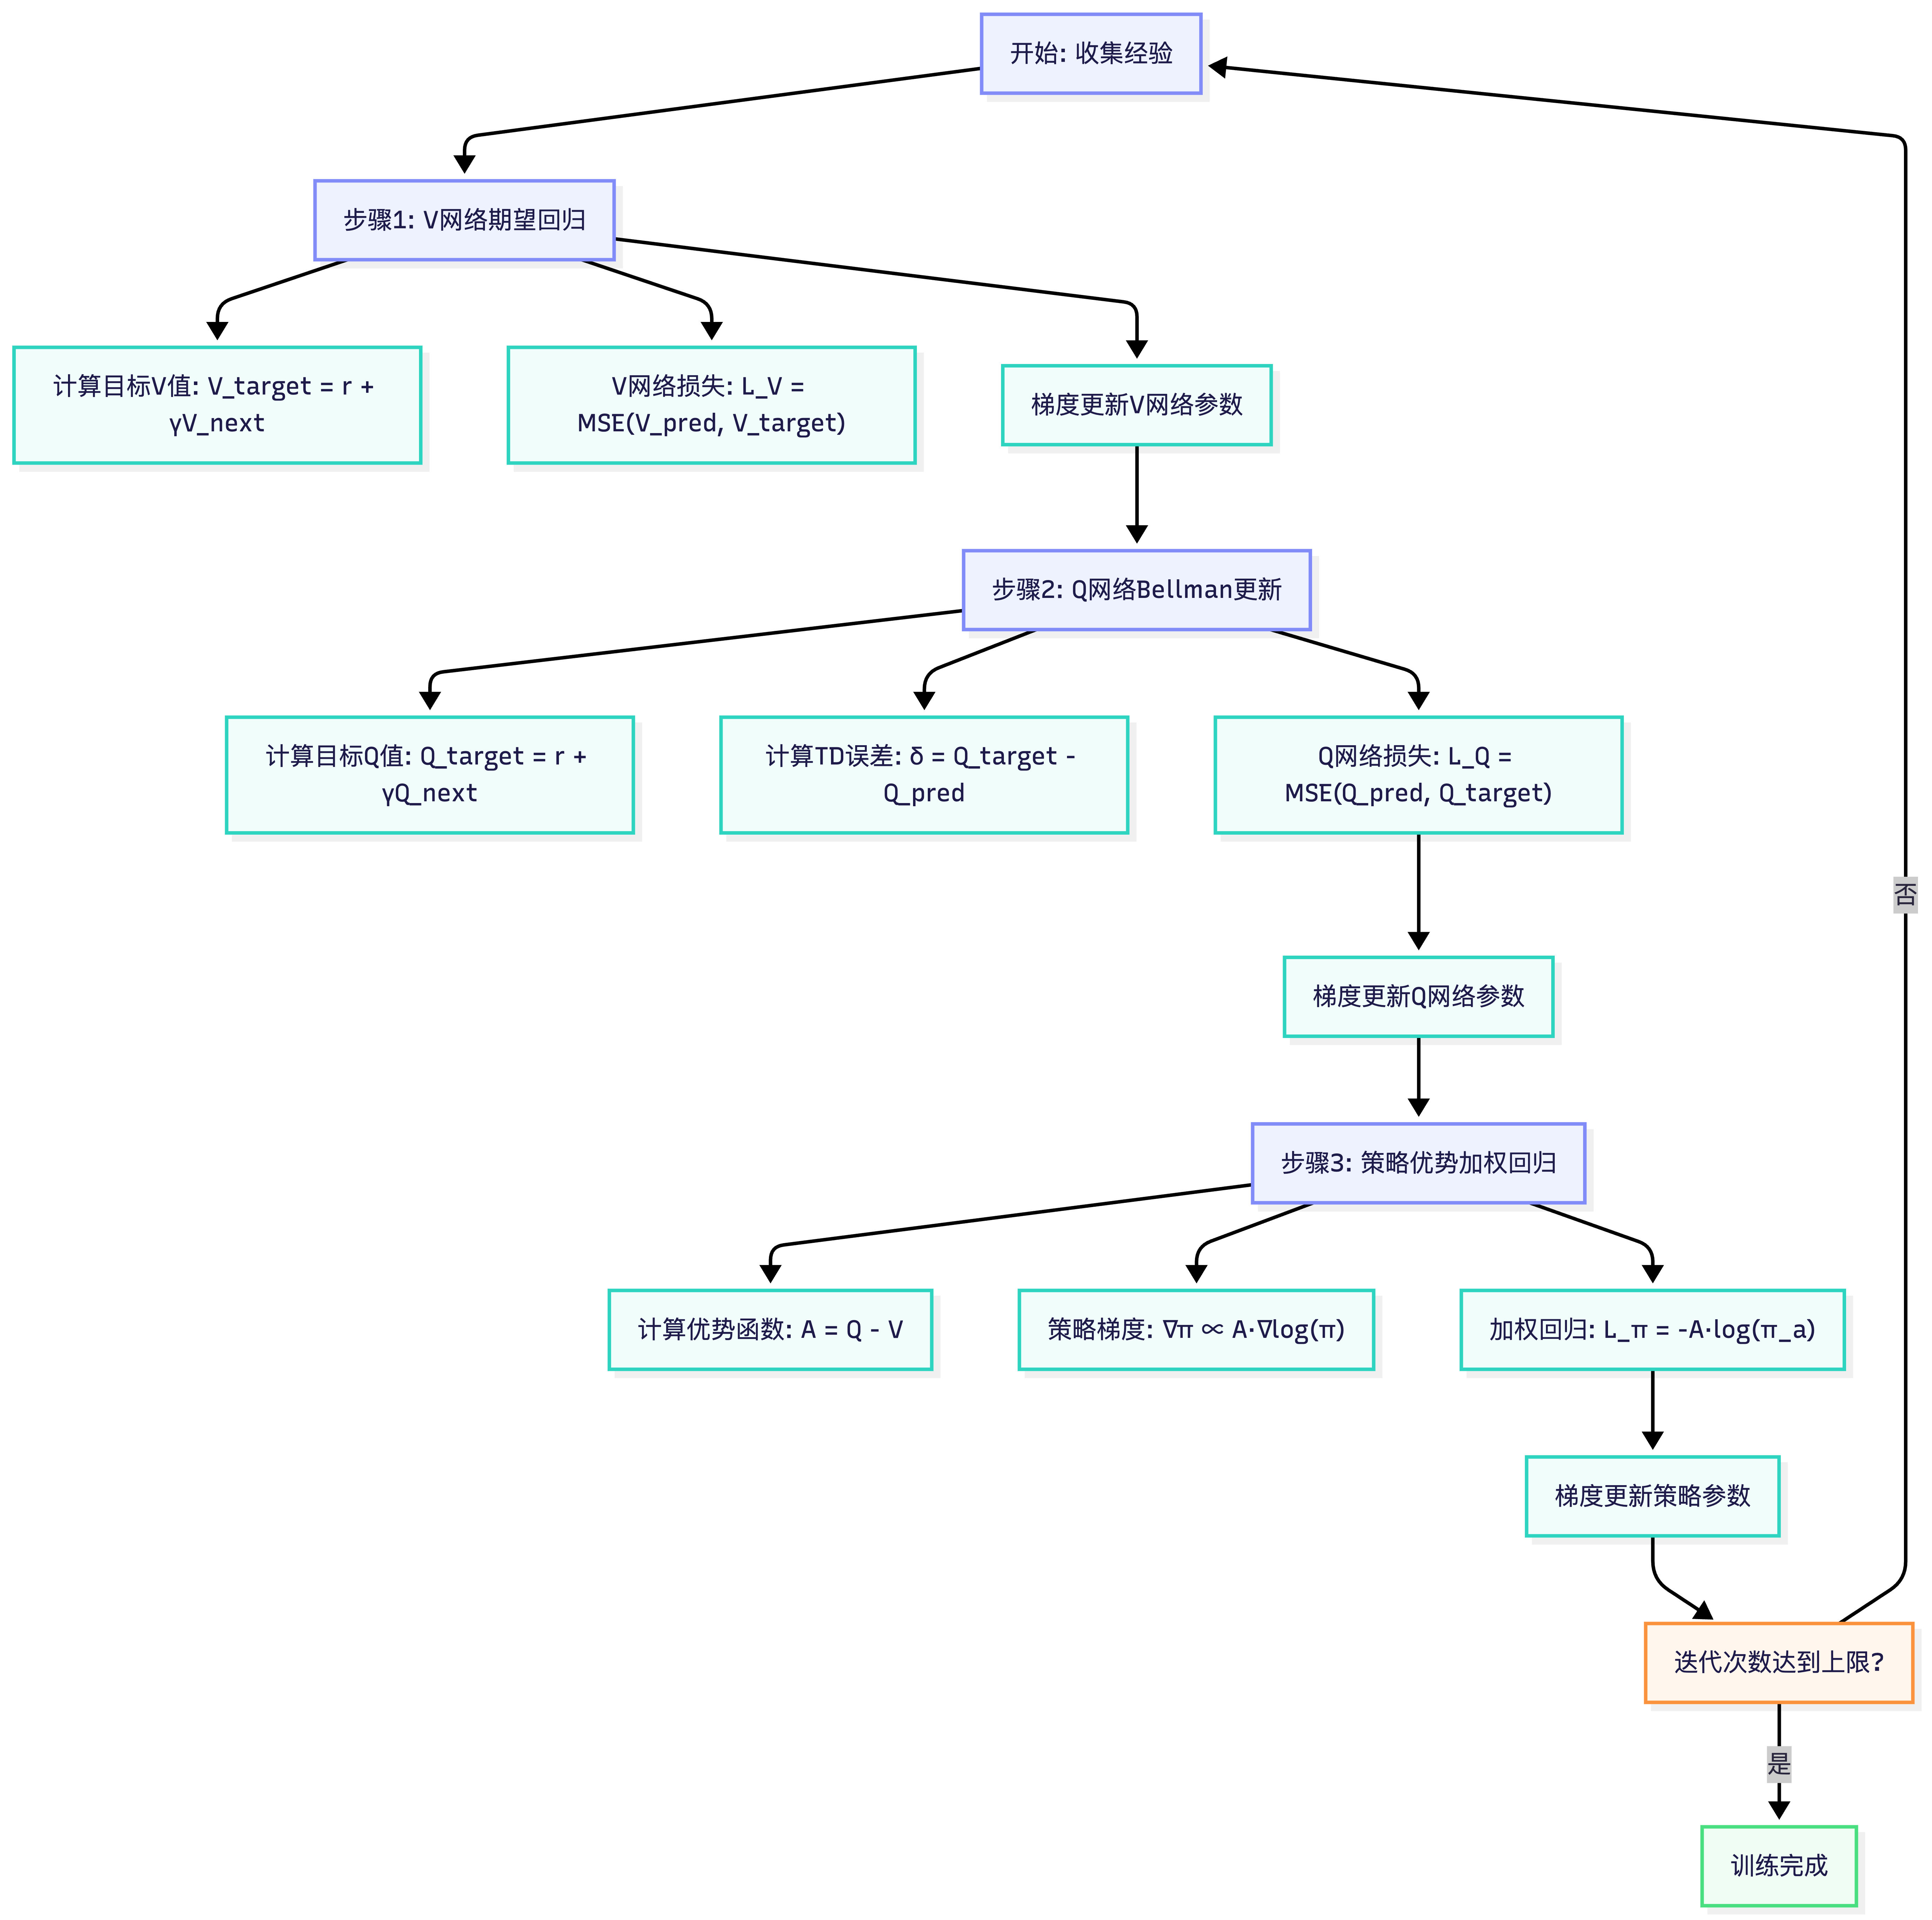
\includegraphics[width=0.5\linewidth]{figures/Targeted_IQL_Training.png}
    \caption{IQL 算法训练流程}
    \label{fig:enter-label}
\end{figure}

\section{本章小结}
本章围绕本文研究所依赖的理论基础与关键技术展开了系统梳理。在 WebRTC 实时通信机制方面，本章剖析了从 SDP 信令协商、ICE 连通性建立到 SRTP 媒体传输的完整协议栈架构，并着重阐述了 Transport-CC 反馈机制在发送端带宽估计中的核心作用——该机制为本文的数据采集平台提供了高频、精准的底层网络状态观测通道。在拥塞控制建模层面，本章形式化定义了 RTC 场景下的多目标 QoE 优化模型，解析了 GCC 算法基于延迟梯度与丢包反馈的双回路耦合控制逻辑，并从无线信道随机性与参数静态性两个维度揭示了启发式规则的结构性瓶颈。在强化学习理论层面，本章建立了从马尔可夫决策过程到离线策略优化的完整数学框架，阐明了离线强化学习中分布偏移问题的根源，并系统推导了隐式 Q 学习（IQL）通过期望回归与非对称损失函数规避分布外动作价值查询的理论机制。上述理论基础为后续章节的数据集构建、模型训练与部署验证提供了不可或缺的技术支撑。